\chapter{Recurrent Neural Networks (RNNs)}
\section{Motivation}

\textbf{Autoencoders} can be used to learn an \textbf{embedding space}.
\begin{itemize}
  \item \textbf{Encoder:}
\(\text{data} \rightarrow \text{embedding}\)
  
  \item \textbf{Decoder:}
\(\text{embedding} \rightarrow \text{data}\)

\end{itemize}

How can we learn \textbf{embedding of words}?\\

\noindent First, we need a way to convert words into numerical features, or in other words, \textbf{turn word features into vectors}. \\

One way to do this is to treat each word as a unique feature (\textbf{integer encoding}):
\begin{itemize}
    \item E.g. cat = 0, dog = 1, or
    \item favourite color: red = 1, blue = 2, green = 3, etc.
\end{itemize}

\begin{definition}
\textbf{Integer Encoding:} technique in data preprocessing and natural language processing (NLP) that involves assigning a unique integer value to each distinct element or category in a dataset. This encoding simplifies the representation of categorical or nominal data, such as words in text or categories in a dataset, by replacing them with corresponding integer IDs.
\end{definition}

The problem with this is that the \textbf{model might assume some relationship between classes solely based on the distance between indices}, while in reality, the numbers are assigned arbitrarily. When there is no specific order, integer encoding is not enough. Assuming an order may lead to \textbf{poor performance}. \\

A better way is to convert word features into numerical features with \textbf{one-hot encoding}. 
\begin{itemize}
    \item For example, at UofT, the categorical feature "Term" can take on three possible values: Fall, Winter, Summer where:
    \begin{itemize}
        \item Fall = [1, 0, 0]; Winter = [0, 1, 0]; Summer = [0, 0, 1]
    \end{itemize}
\end{itemize}

\begin{definition}
\textbf{One-hot Encoding:} a data preprocessing technique used in machine learning and data analysis. It converts categorical data, such as discrete categories or labels, into a binary vector representation. Each category is represented as a binary vector where all elements are zero except for one, which corresponds to the category being "hot" or "on."
\end{definition}

\begin{itemize}
    \item This is better than integer encoding in the way that there is no superficial relationship created between the words, however, there are two significant problems:
\end{itemize}
\begin{enumerate}
    \item \textbf{Dimensions grow with the number of words}: eg. 10000 words means 10000 dimensional encoding!
    \item \textbf{One-hot encoding assumes each word is completely independent}: cannot model relative similarities between words
\end{enumerate}


\section{Word Embeddings}
How can we achieve word embedding?
\begin{itemize}
  \item Words are different from images
  \item Characters are not like pixels in images
  \item The \textbf{meaning of a word} is not represented by the letters that make up the word
  \item Meaning comes from the sequence of characters and how they are used in conjunction with other words
  \item \textbf{Meaning comes from context}
\end{itemize}
Word Embedding models were created to address this problem. \\
The term Word embedding was coined in 2003 (Bengio et al.)
Two commonly used models:
\begin{itemize}
  \item \textbf{word2vec} model proposed in 2013 (Mikolov et al.)
  \item \textbf{GloVe} vectors released in 2014 (Pennington et al.)
\end{itemize}

\noindent\textbf{Training Word Embeddings}
\begin{itemize}
    \item Encoder: word(??) → embedding
    \item Decoder: embedding → ???
\end{itemize}
\indent Two things to consider:
\begin{enumerate}
    \item How do we encode the word?
    \item What is our target?
\end{enumerate}

\noindent\textbf{One-Hot Encoding of Words}
\begin{itemize}
    \item Each word has its own index
    \item If there are 10,000 words, there are 10,000 features
    \item “happy” → [0, 0, 0, 0, ... , 1, ... , 0, 0, 0, 0]
    \item One-hot embedding as input to the encoder
    \item Encoder: one-hot embedding → low dim embedding
    \item Decoder: low-dim embedding → ???
\end{itemize}
This is a possible solution to the encoding problem but what is our target?\\

\noindent\textbf{Text as Sequences}
\begin{idea}
    The meaning of a word depends on its context, or other words that appear nearby.
\end{idea}
There is evidence that children learn new words based on their surrounding words.\\

\textbf{Architecture of word2vec}
\begin{itemize}
    \item Encoder: one-hot embedding → low-dim embedding
    \item Decoder: low-dim embedding → nearby words
\end{itemize}

\begin{figure}[h!t]
    \centering
    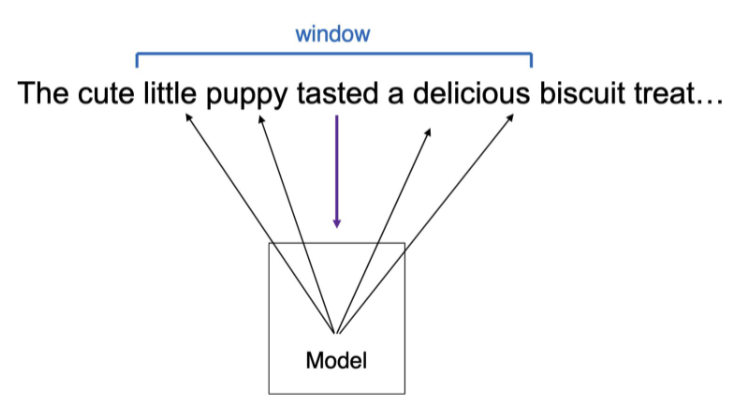
\includegraphics[width=0.5\linewidth]{architectureofword2vec.png}
    \caption{Architecture of word2vec model}
    \label{fig:enter-label}
\end{figure}
\begin{idea}
    The concept of a sliding window is similar to sliding a kernel across an image in CNN.
\end{idea}

The middle word of the window is passed into the model as input and the model tries to predict the context around that word (surrounding words).\\

\noindent\textbf{word2vec}
\begin{definition}
    \textbf{word2vec}: a family of architecture used to learn word embeddings.
\end{definition}
\begin{itemize}
    \item \textbf{Skip-Gram} → Predict context from target (center word as input, context, or surrounding words, as output)
    \item \textbf{CBOW (Continuous Bag of Words)} → Predict target from context (context as input, center word as output)
\end{itemize}

\begin{figure}[h!t]
    \centering
    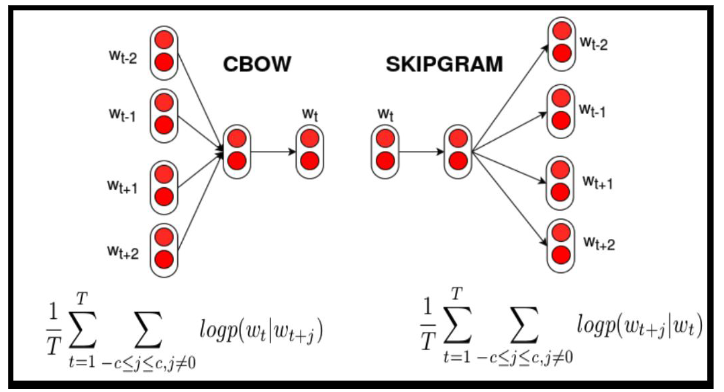
\includegraphics[width=0.75\linewidth]{skipgramcbow.png}
    \caption{CBOW and Skipgram Architectures}
    \label{fig:enter-label}
\end{figure}

\textbf{Skip-Gram Model}
\begin{itemize}
    \item Predict context words from target words
    \item Components don't need to be consecutive in the text'
    \item Can be skipped over or randomly seleted from many documents
\end{itemize}

\begin{definition}
    \textbf{n-Gram:} a contiguous  sequence of n items from a given text.
\end{definition}

\begin{definition}
    \textbf{k-Skip n-Gram:} an n-gram that can involve a skip operation of size k or smaller.
\end{definition}

\begin{figure}[h!t]
    \centering
    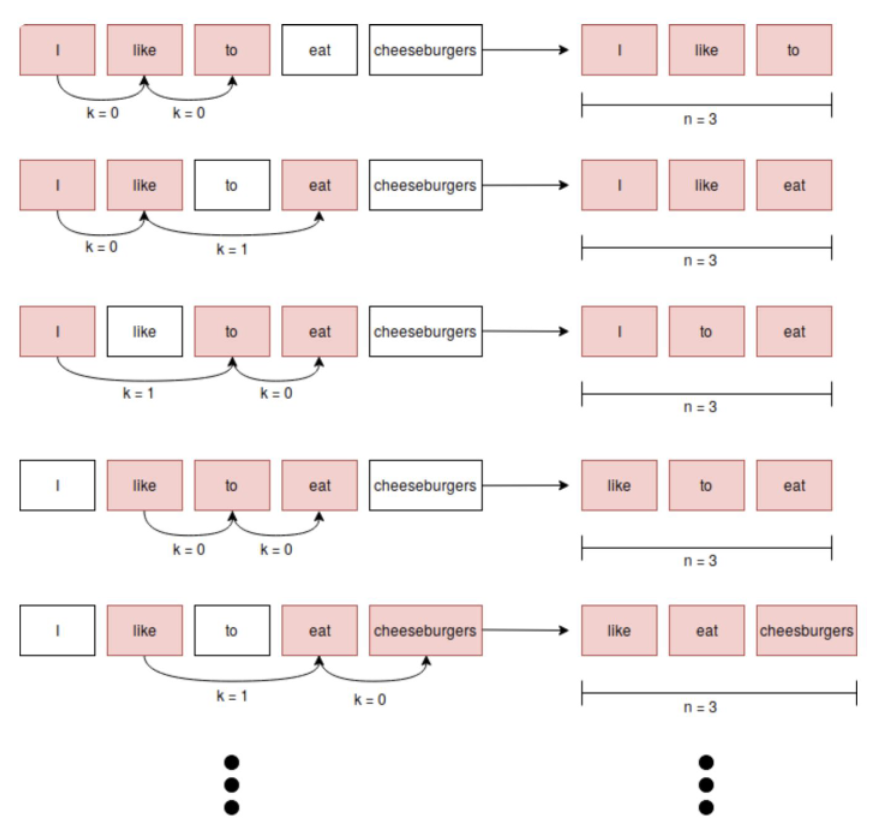
\includegraphics[width=0.75\linewidth]{1skip3gram.png}
    \caption{1-Skip 3-Gram}
    \label{fig:enter-label}
\end{figure}

\begin{idea}
    Skip-Gram: Given a word predict its neighbouring words.
\end{idea}

\begin{itemize}
    \item The number of neighboring words are defined by the window size, which is a hyper-parameter.
\end{itemize}
\begin{figure}[h!t]
    \centering
    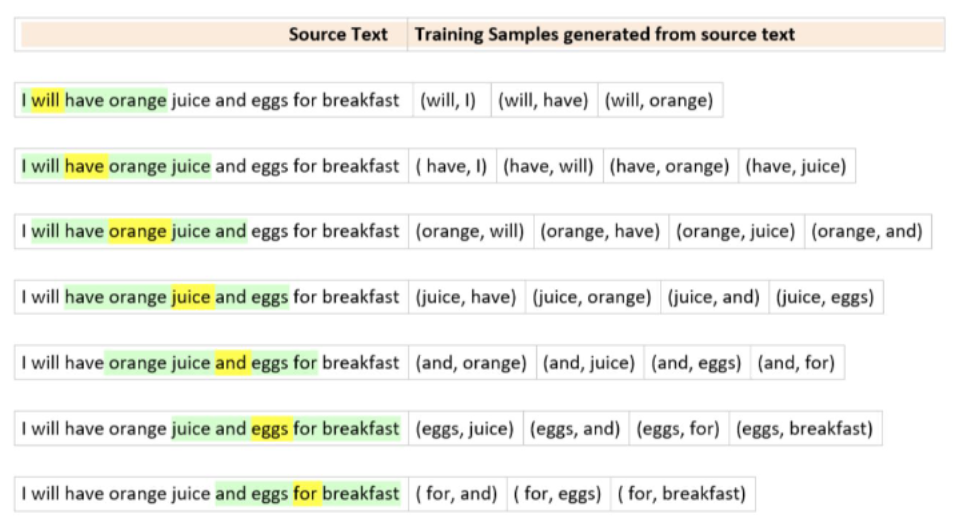
\includegraphics[width=0.65\linewidth]{neighbouringwords.png}
    \caption{Skip-Gram neighbouring words}
    \label{fig:enter-label}
\end{figure}

\begin{figure}
    \centering
    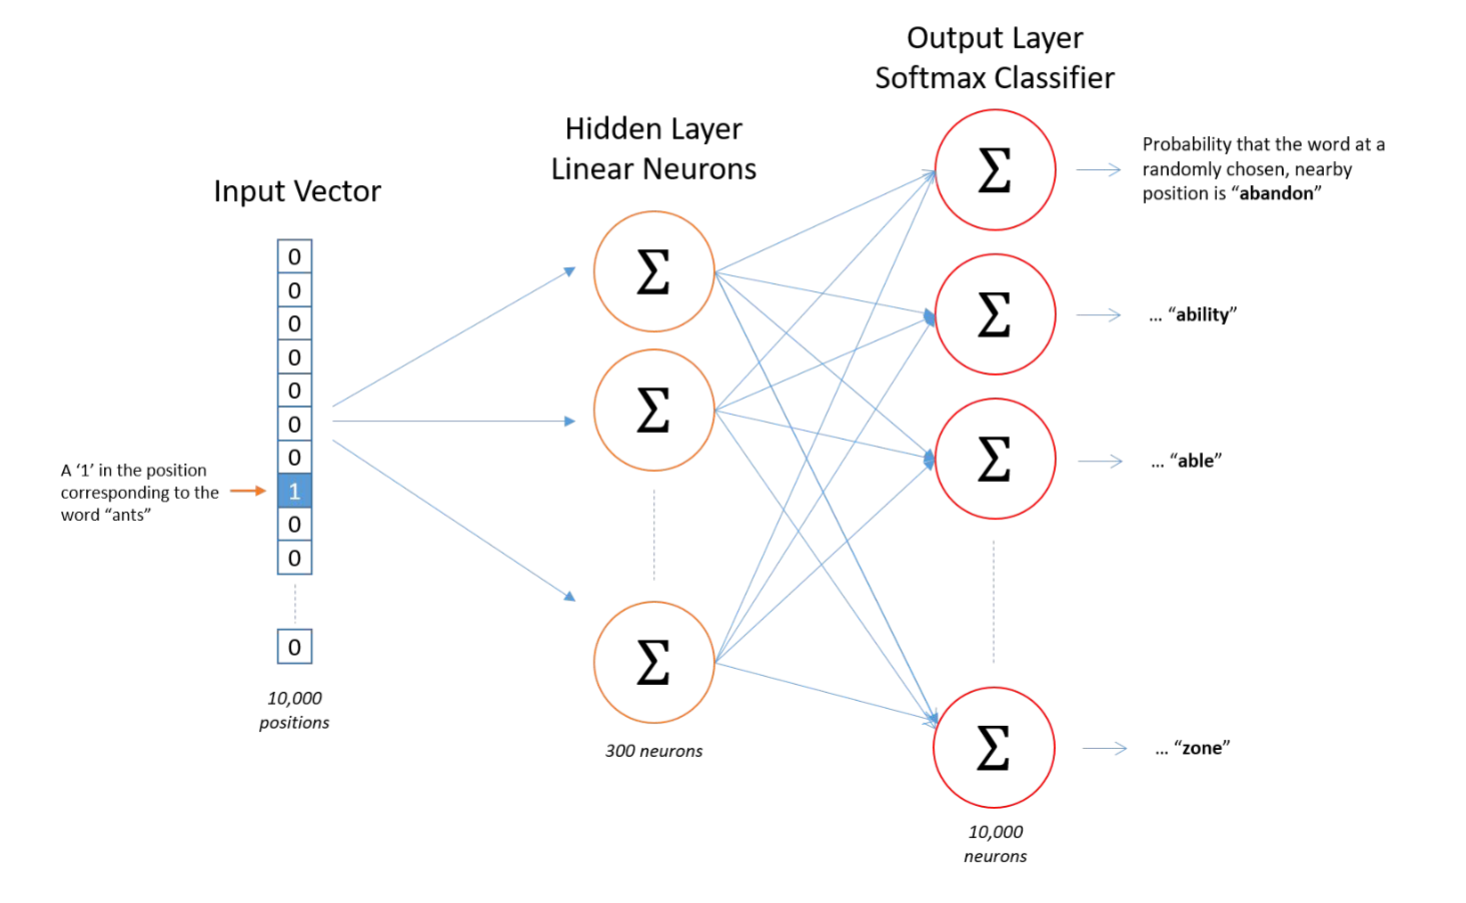
\includegraphics[width=1\linewidth]{skipgramarc.png}
    \caption{Skip-Gram Architecture}
    \label{fig:enter-label}
\end{figure}

\begin{itemize}
    \item The output layer is only used for training
    \item After the model is trained, we only keep the weights from input to hidden layer
    \item Words that have similar context words will be mapped to similar embeddings
\end{itemize}

\newpage

\textbf{Continuous Bag of Words (CBOW) Model}

\begin{itemize}
    \item Predicts the center word from a fixed window size of context words
    \item Note that similar to SkipGram model, the input and output to the model are one-hot representation of pair of words
\end{itemize}

\textbf{CBOW Vs Skip-Gram}\\

Skip-Gram:
\begin{itemize}
  \item Works well with small datasets
  \item Better semantic relationships (cat \& dog)
  \item Better representation of less frequent words
\end{itemize}

CBOW:
\begin{itemize}
  \item Trains faster than Skip-Gram as the task is simpler
  \item Better syntactic relationships (cat \& cats)
  \item Better representation of more frequent words
\end{itemize}

\begin{idea}
    The biggest limitation of word2vec is that the model is constrained to windows of text.
\end{idea}

\newpage

\noindent \textbf{GloVe}\\

\\Word2Vec does not have any explicit global information. GloVe enforces global information into the embeddings:

\begin{itemize}
    \item Compute\textbf{ co-occurrence frequency counts }for each word, represented as a
matrix where element X ij denotes the number of times word i appears in
the context of word j
\begin{itemize}
    \item Number of times when words are associated each other is counted
\end{itemize}
\item \textbf{Optimization:} Inner product of word vectors should be a good predictor
of co-occurrence frequency

\begin{figure}[h!t]
    \centering
    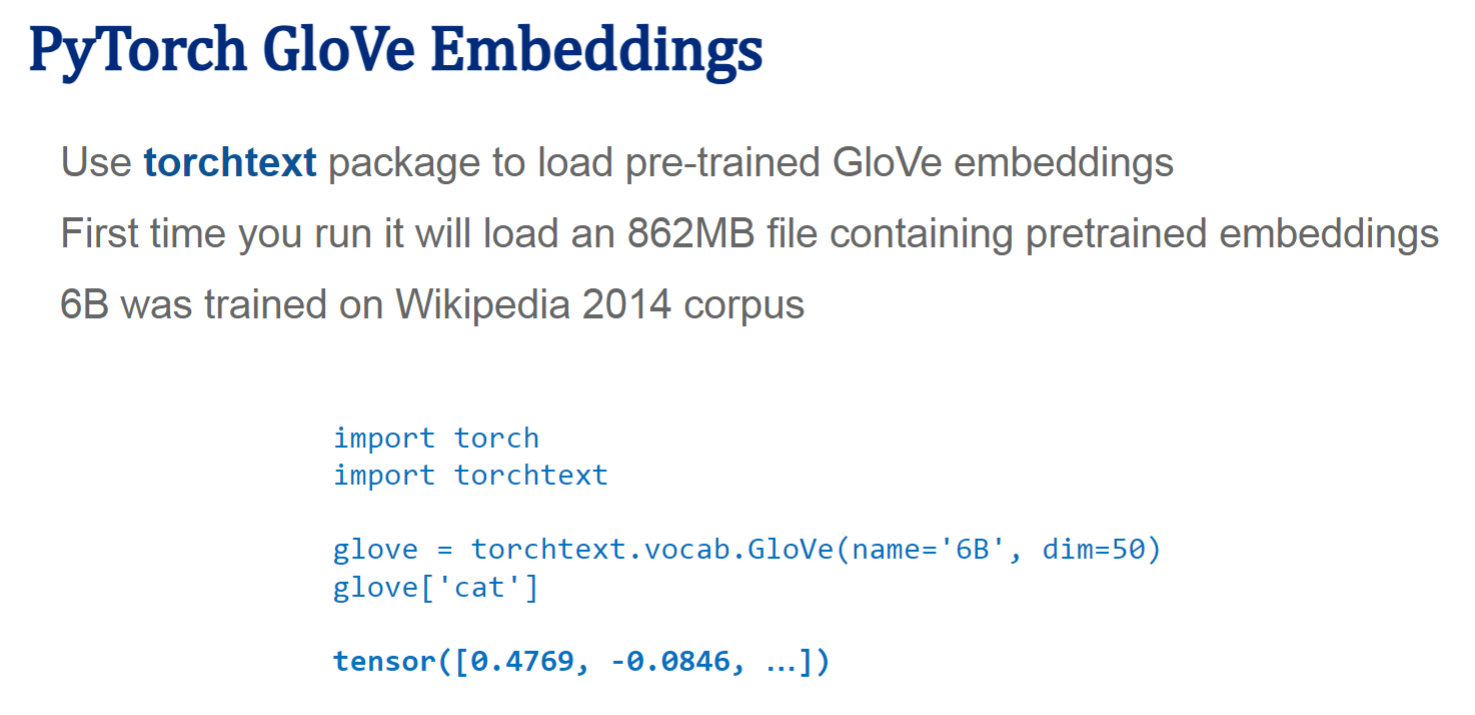
\includegraphics[width=0.75\linewidth]{gloveembpy.png}
    \caption{PyTorch GloVe Embeddings}
    \label{fig:enter-label}
\end{figure}
\end{itemize}

Distance measures will allow us to measure the distance between embeddings.

\section{Distance Measures}

In order to talk about which words have similar embeddings, we need to
introduce a measure of distance in the embedding space:
\begin{itemize}
  \item \textbf{Euclidean Distance} $\rightarrow$ L2-norm of embeddings (sensitive to magnitude)

\[ D(\vec{X}, \vec{Y}) = || \vec{X} - \vec{Y} || = \sqrt{\sum_{i=0}^{d}(x_i - y_i)^2}\]

  \item \textbf{Cosine Similarity} $\rightarrow$ cosine of the angle between embeddings (invariant to magnitude)
\end{itemize}


\[ Similarity(\vec{X}, \vec{Y}) = cos(\theta) = \frac{{\mathbf{\vec{X}} \cdot \mathbf{\vec{Y}}}}{{\|\mathbf{\vec{X}}\| \cdot \|\mathbf{\vec{Y}}\|}} = \frac{{\sum_{i=0}^{d} x_i \cdot y_i}}{{\sqrt{\sum_{i=0}^{d} x_i^2} \cdot \sqrt{\sum_{i=0}^{d} y_i^2}}}\]

\begin{figure}[h!t]
    \centering
    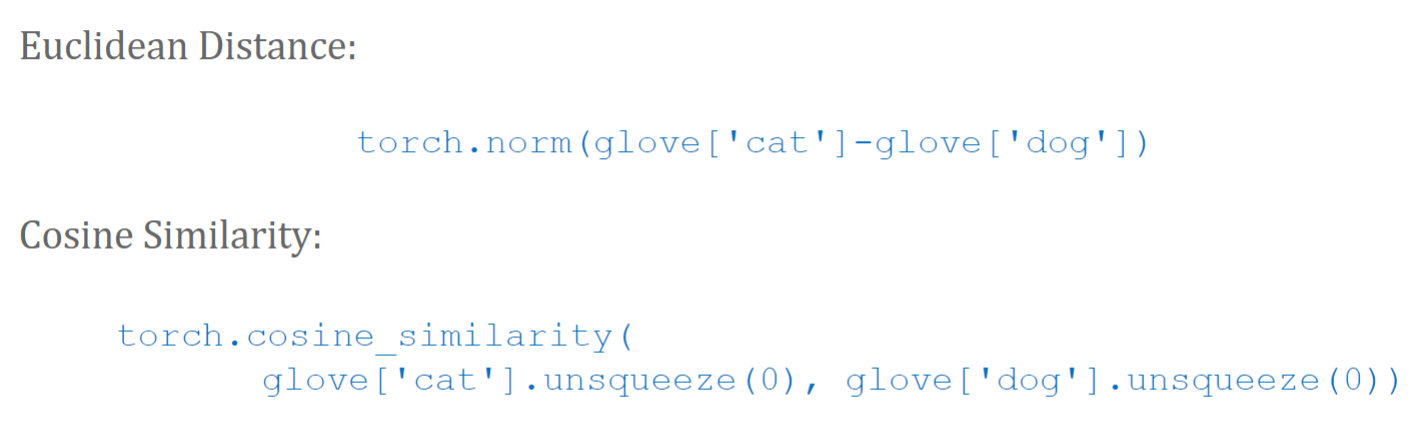
\includegraphics[width=0.9\linewidth]{distancepy.png}
    \caption{Computing Distance in PyTorch}
    \label{fig:enter-label}
\end{figure}

\newpage

\noindent
\textbf{Word Analogies}\\
One surprising thing about the embedding space is the extent of its structure.\\
We often see relationships like this in GloVe embeddings:

\begin{figure}[h!t]
    \centering
    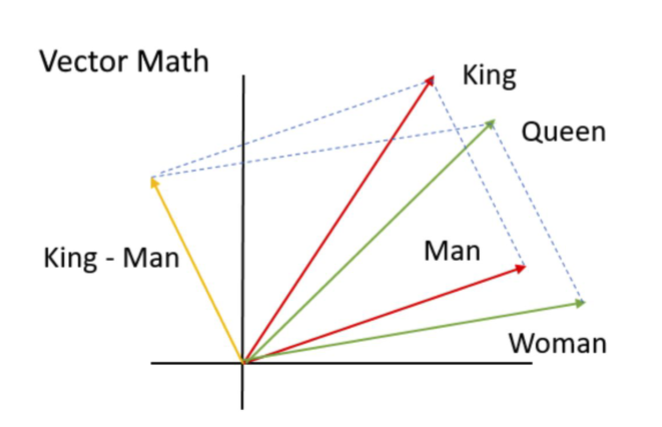
\includegraphics[width=0.7\linewidth]{gloverelationships.png}
    \caption{Showing bias of models}
    \label{fig:enter-label}
\end{figure}

\begin{idea}
    This word analogies show that machine learning models are not unbiased. 
\end{idea}
\begin{warning}
    Machine learning models learn the biases present in the data it is trained on. The distance between embeddings is trained according to these biases.
\end{warning}

\section{Language Models}

\begin{definition}
    \textbf{Language Models:} neural network-based algorithms designed to understand and generate human language text. They use vast amounts of text data to learn the statistical patterns and relationships within language, enabling tasks such as text generation, translation, summarization, and sentiment analysis. These models have revolutionized natural language processing by providing powerful tools for various language-related tasks.
\end{definition}

\noindent\textbf{Learning probability distribution over sequences of words}
\begin{itemize}
    \item \textbf{Text Understanding}
    \begin{itemize}
        \item Question Answering
        \item Sentiment Analysis
    \end{itemize}
    \item \textbf{Text Generation}
    \begin{itemize}
        \item Sentence completion
        \item Generating captions, sentences, stories. . .
        \item Translation
    \end{itemize}
    \item . . . and more!
\end{itemize}

\noindent \textbf{How is working with text different (more challenging) from working with images?}
\begin{itemize}
    \item Grammar, spelling
    \item Many words to learn
    \item Choice of working with words vs characters
    \item Arbitrary length input / output
    \item Different languages
\end{itemize}

\noindent\textbf{Sentiment Analysis}\\

The goal of sentiment analysis is to identify the sentiment a text conveys. It can be applied to:
\begin{itemize}
    \item Movie reviews
    \item Product feedback
    \item Emails
    \item Tweets

\end{itemize}

\begin{figure}[h!t]
    \centering
    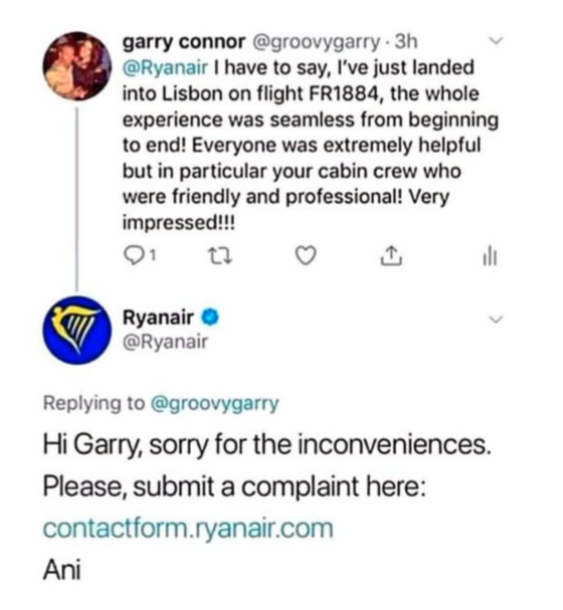
\includegraphics[width=0.5\linewidth]{failingsentimentanalysis.png}
    \caption{Sentiment Analysis Fail}
    \label{fig:enter-label}
\end{figure}

\noindent\textbf{Dataset: Sentiment140}\\

1,600,000 tweets collected by students doing a course project where sentiment determined by emoticon $\rightarrow$ :) positive and :( negative. For each tweet in the training data, we will:
\begin{enumerate}
    \item Split the tweet into words
    \item Look up the GloVe embedding for each word, ignoring words that don't have embeddings
    \item Add up the word embeddings to obtain an embedding for the entire tweet
    \item The tweet embedding will be the input to a fully-connected neural network
\end{enumerate}

\textbf{Limitations:} These two sentences will have the same embedding in our model:
\begin{itemize}
    \item The food was adequate, but just not great
    \item The food was not just adequate, but great
\end{itemize}
But they have drastically different meanings. Our model does not take into account the order of words; the summation operation causes the data to lose the order of the words. How can we do better?\\

\textbf{Idea 1}:
Concatenate the word embeddings, then train a neural network that takes the concatenated embedding as input.
\begin{itemize}
    \item While the order of the data is maintained, there are two main issues with this method:
\end{itemize}

\begin{enumerate}
    \item Input to the fully-connected network will not be consistent
    \item If we try to use padding techniques to problem 1, then we will have an extremely high number of parameters
\end{enumerate}

\begin{figure}[h!t]
    \centering
    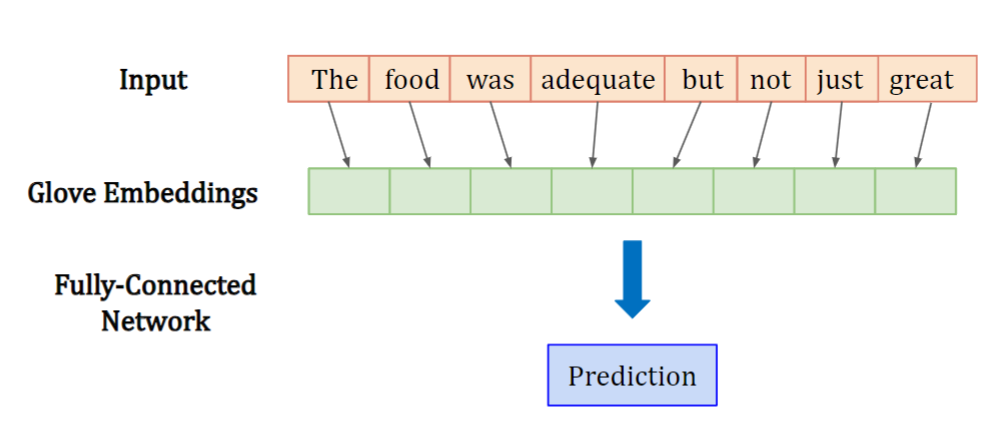
\includegraphics[width=0.75\linewidth]{rnnidea1.png}
    \caption{Sentiment140 Idea 1}
    \label{fig:enter-label}
\end{figure}

\textbf{Idea 2}:
Concatenate the word embeddings, then train a 1-dimensional convolutional neural network that takes the concatenated embedding as input.
\begin{itemize}
\item This addresses the sizing issue, however this presents a new issue that has to do with the nature of convolution.
    \item \textbf{Convolution is local}: this means that the model will miss the long range dependency that comes with sentences. Elements (words) that are away from each other in a string may still be highly dependent on each other for context.
\end{itemize}

\begin{figure}[h!t]
    \centering
    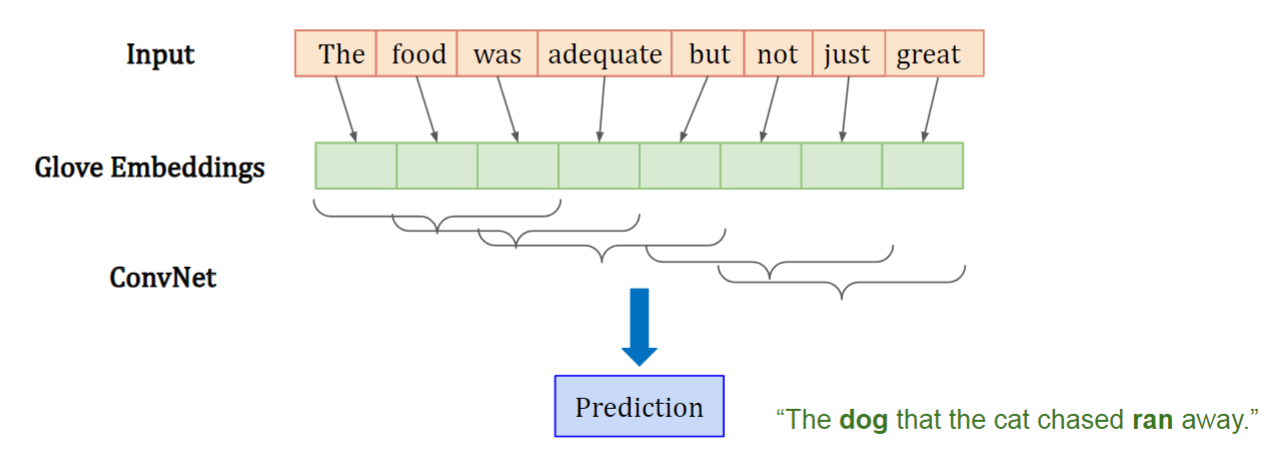
\includegraphics[width=1\linewidth]{rnnidea2.png}
    \caption{Sentiment140 Idea 2}
    \label{fig:enter-label}
\end{figure}

We need recurrent neural networks to address these issues.

\section{Recurrent Neural Networks}
\textbf{Idea 3:} Use a recurrent neural network
\begin{itemize}
    \item Can take in variable-sized sequential input
    \item Can remember things over time, or has some sort of \textbf{memory or state}
\end{itemize}

\begin{figure}[h!t]
    \centering
    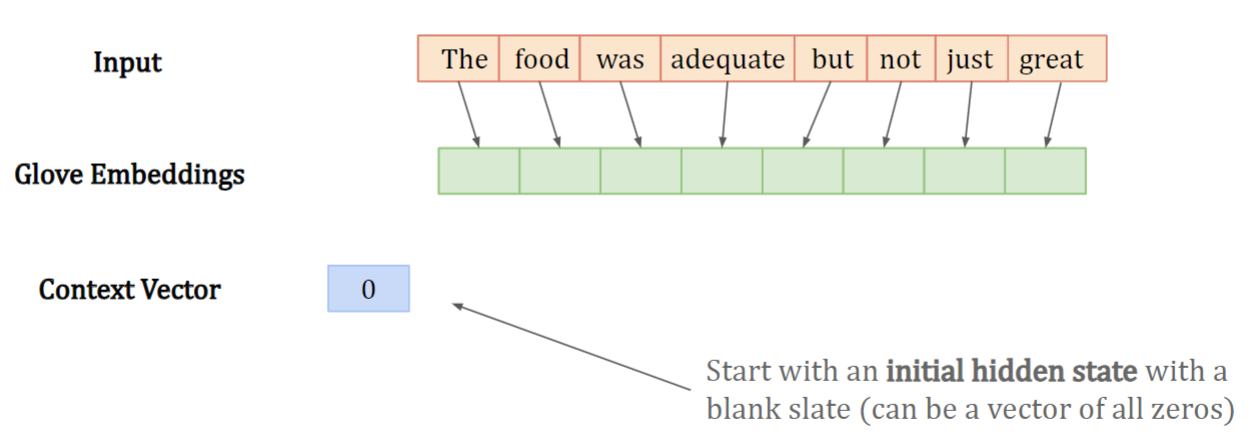
\includegraphics[width=0.9\linewidth]{rnnidea3.png}
    \caption{Sentiment140 Idea 3}
    \label{fig:enter-label}
\end{figure}

\begin{definition}
    \textbf{Context Vector:} a fixed-size representation that summarizes the information from the entire input sequence processed by the RNN. It captures the context or relevant information from past time steps and serves as an input to subsequent parts of the network, allowing the RNN to maintain memory and make predictions based on the entire sequence history.
\end{definition}

\textbf{Updating Hidden State:} hidden state is updated based on previous hidden state and the input using the
same neural network as before (weight sharing).\\

\begin{itemize}
    \item The hidden state is updated until we run out of tokens.

\begin{figure}[h!t]
    \centering
    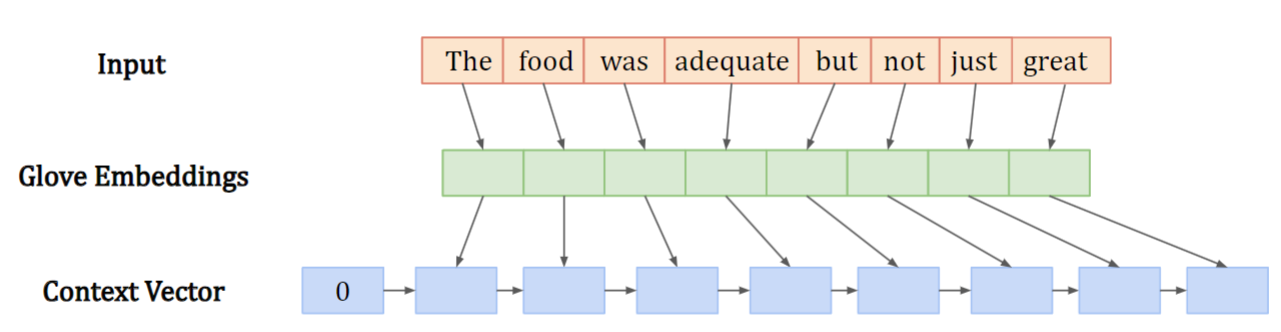
\includegraphics[width=0.75\linewidth]{updatinghiddenstate1.png}
    \caption{Updating hidden state}
    \label{fig:enter-label}
\end{figure}

    \item The last hidden state is used as input to a prediction network (fully-connected network).

\begin{figure}[h!t]
    \centering
    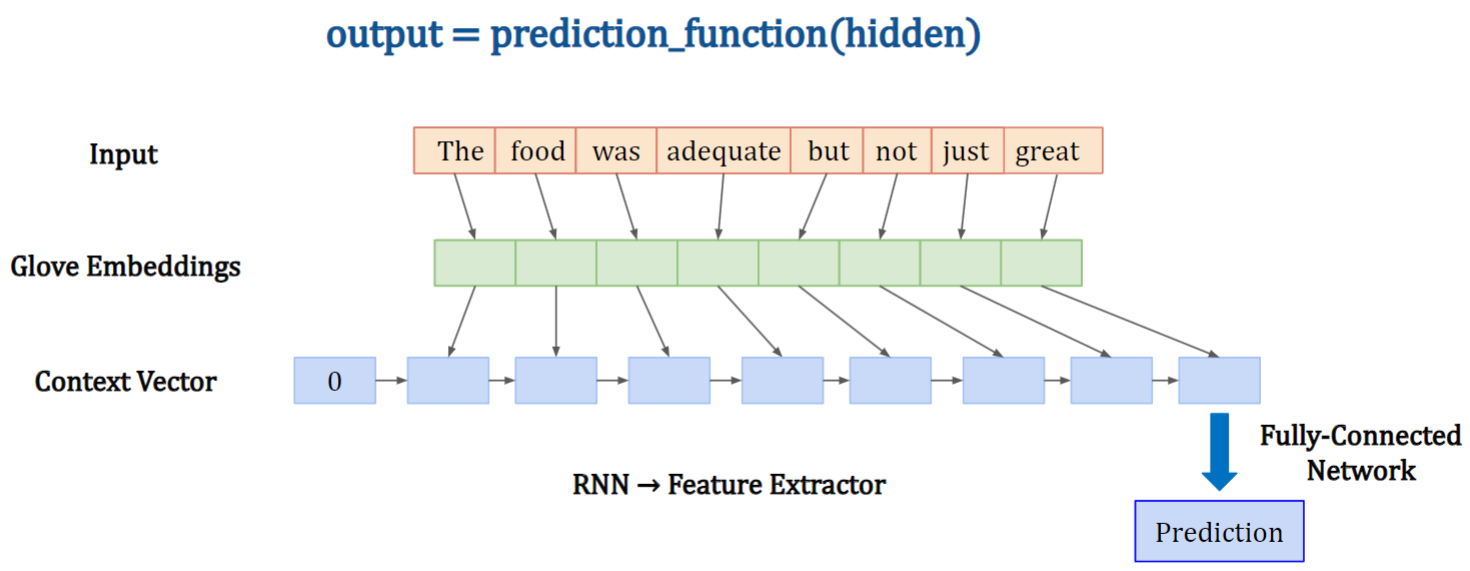
\includegraphics[width=0.75\linewidth]{updatehiddenstate2.png}
    \caption{Last hidden state into classifier}
    \label{fig:enter-label}
\end{figure}

    \item RNN layers have a recursive process that we have not seen in any other type of network so far.
\end{itemize}

\begin{figure}[h!t]
    \centering
    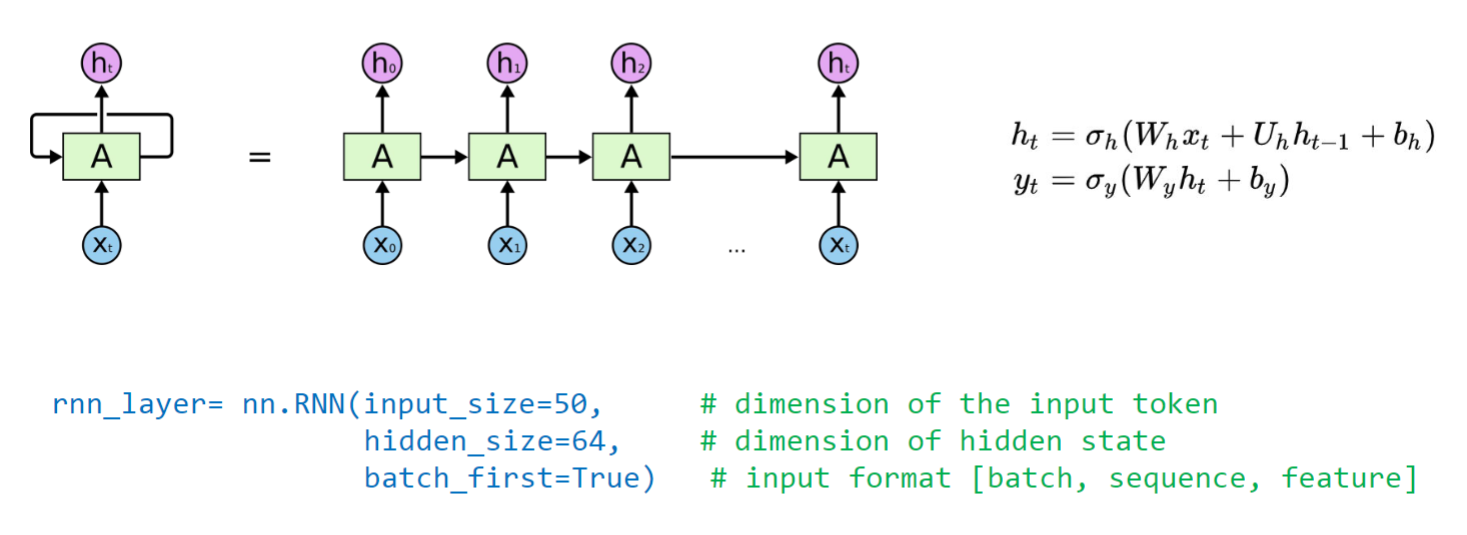
\includegraphics[width=1\linewidth]{rennrecursion.png}
    \caption{RNN layers visualized (unrolled)}
    \label{fig:enter-label}
\end{figure}


\begin{idea}
    RNN uses its past to determine its future. Many real world problems deal with inputs/outputs with varying sizes and require data from the past to accurately model future data.
\end{idea}

\begin{figure}
    \centering
    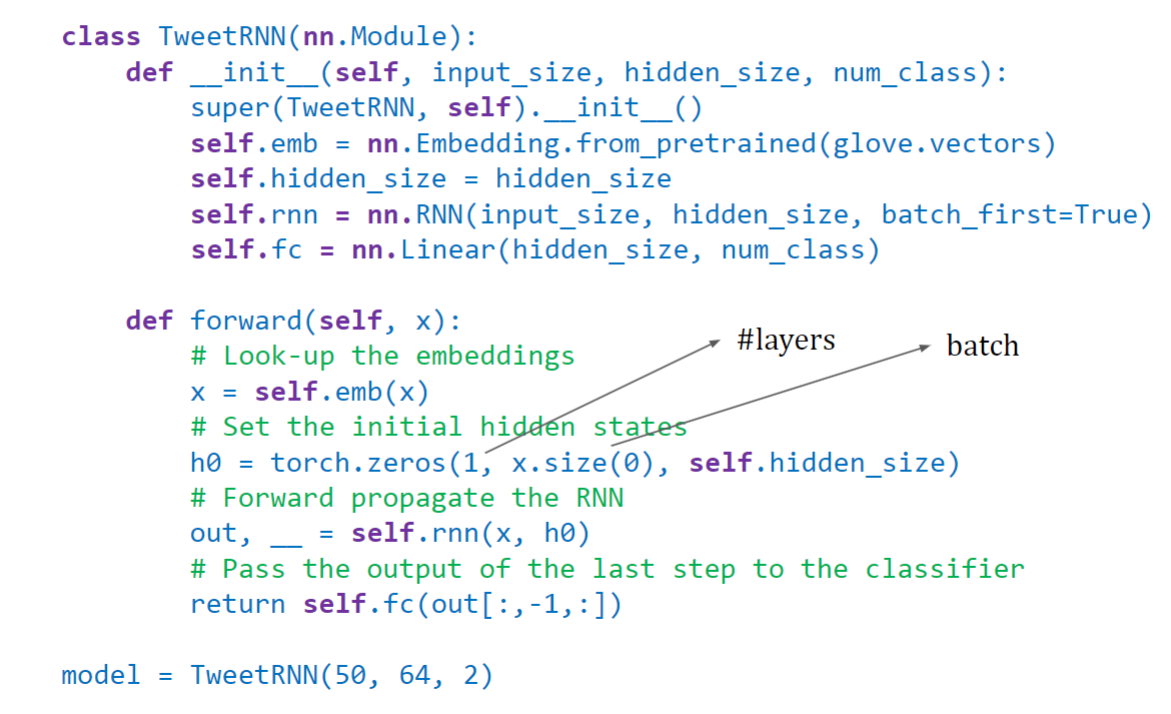
\includegraphics[width=1\linewidth]{rnnarc.png}
    \caption{PyTorch implementation of RNN (Training code is similar to previous architectures)}
    \label{fig:enter-label}
\end{figure}

If we consider the concatenated input/hidden and output/hidden vectors as simply input/output, forward path in RNN is simply a fully-connected NN.

\begin{figure}[h!t]
    \centering
    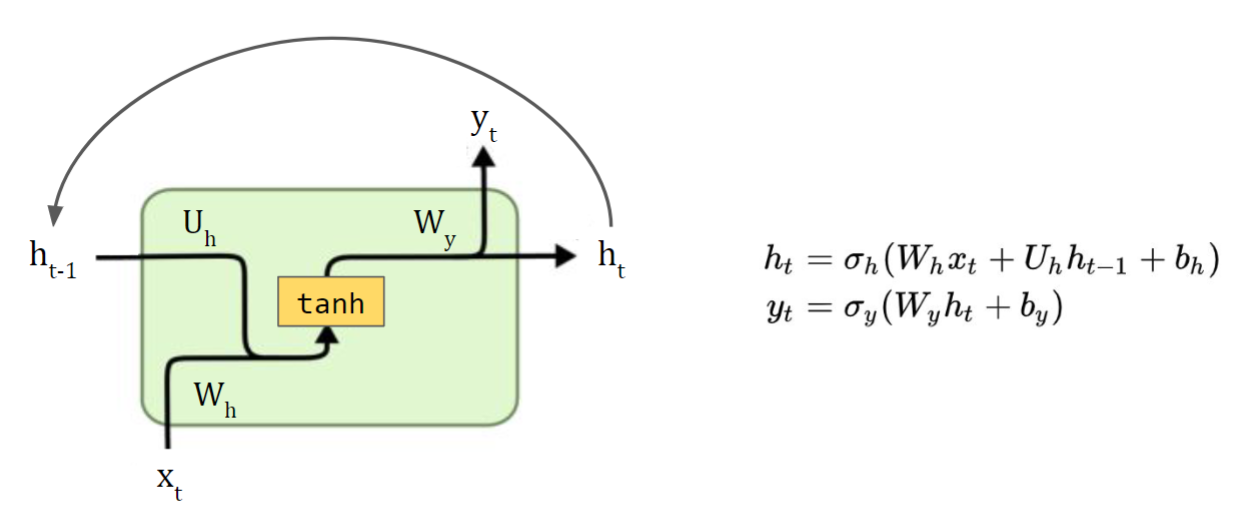
\includegraphics[width=1\linewidth]{rnnforwardpath.png}
    \caption{Forward path of RNN as a fully-connected NN}
    \label{fig:enter-label}
\end{figure}

\begin{figure}[h!t]
    \centering
    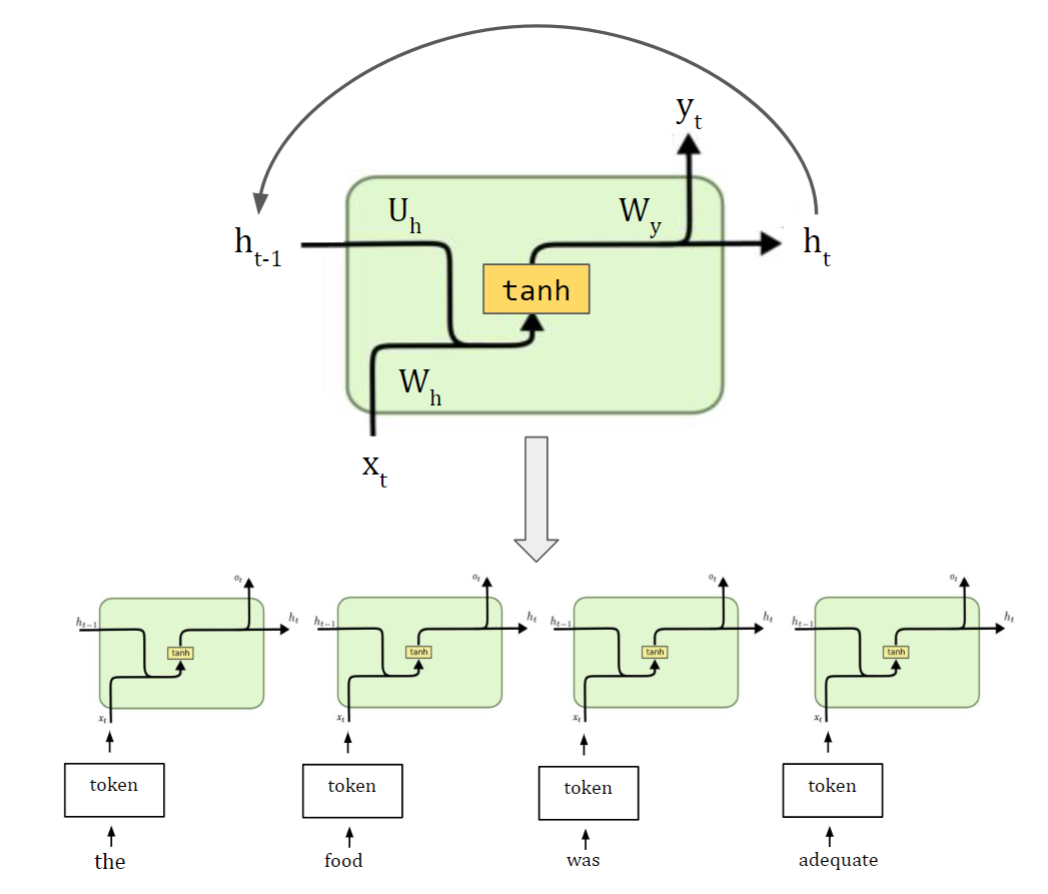
\includegraphics[width=0.75\linewidth]{unrolledrnn.png}
    \caption{Unrolling an RNN}
    \label{fig:enter-label}
\end{figure}

\newpage

\textbf{Sequence-Level Predictions}
\begin{figure}[h!t]
    \centering
    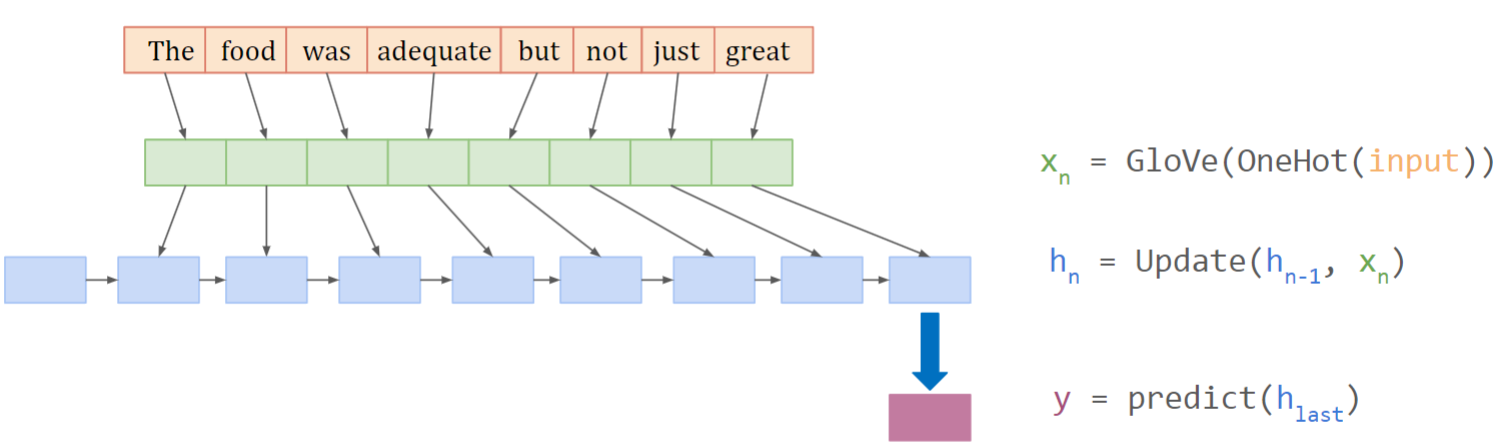
\includegraphics[width=1\linewidth]{sequencelevelpredictions.png}
    \caption{Sequence-Level Predictions}
    \label{fig:enter-label}
\end{figure}
\begin{itemize}
    \item  These come into play when the goal is to make predictions or decisions based on the \textbf{entire sequence as a whole}. 
    \item This is common in tasks like text summarization, machine summarization, or sequence-to-sequence tasks like language translation. 
    \item In these cases, the model generates an output sequence that summarizes or transforms the input sequence, and the quality of the entire generated sequence is assessed rather than individual tokens.
\end{itemize}

\newpage

\textbf{Token-Level Predictions}

\begin{figure}[h!t]
    \centering
    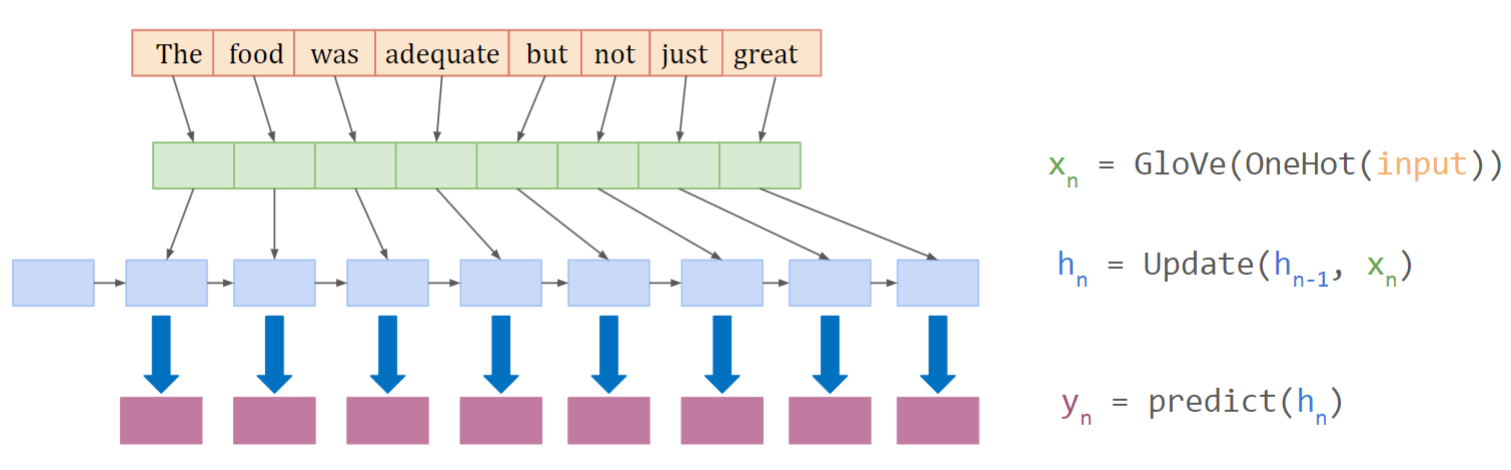
\includegraphics[width=1\linewidth]{tokenlevelpredictions.png}
    \caption{Token-Level Predictions}
    \label{fig:enter-label}
\end{figure}

\begin{itemize}
    \item These are employed when you need predictions or labels for \textbf{individual elements within a sequence}, such as words in a sentence or characters in a text. 
    \item Token-level predictions are useful for tasks like part-of-speech tagging, named entity recognition, sentiment analysis, and machine translation, where you want to annotate or classify each element independently within the sequence
\end{itemize}
\section{Limitations of Vanilla RNNs}

What happens to RNNs unrolled onto a \textbf{long sequence}?
\begin{itemize}
    \item RNNs can be very \textbf{deep} $\rightarrow$ Depth = Length of sequence
\end{itemize}

There are two related problems with vanilla RNNs:
\begin{itemize}
    \item Not good at modelling \textbf{long-term dependencies}
    \item Hard to train due to \textbf{vanishing/exploding gradients}\\
\end{itemize}

\noindent \textbf{Exploding/Vanishing Gradients}\\

\begin{figure}[h!t]
    \centering
    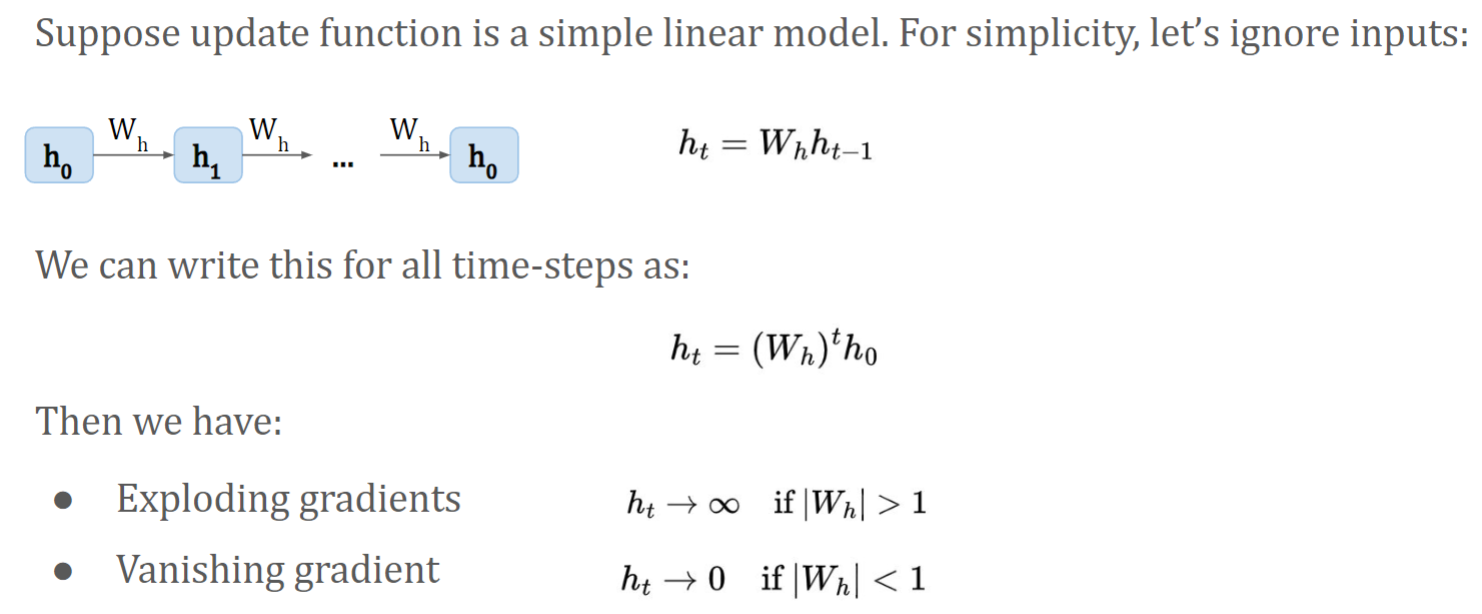
\includegraphics[width=0.75\linewidth]{explodingvanishinggrads.png}
    \caption{Exploding and Vanishing Gradients}
    \label{fig:enter-label}
\end{figure}

\textbf{Gradient clipping $\rightarrow$ Exploding Gradient}
\begin{itemize}
    \item If gradient is greater than a threshold, set the gradient to threshold
\end{itemize}

\textbf{Skip-connection $\rightarrow$ Vanishing Gradient}
\begin{itemize}
    \item Ideally we want skip connections to all previous states $\rightarrow$ Too expensive
    \item We could preserve the hidden state/context over the long term
\end{itemize}

\begin{figure}[h!t]
    \centering
    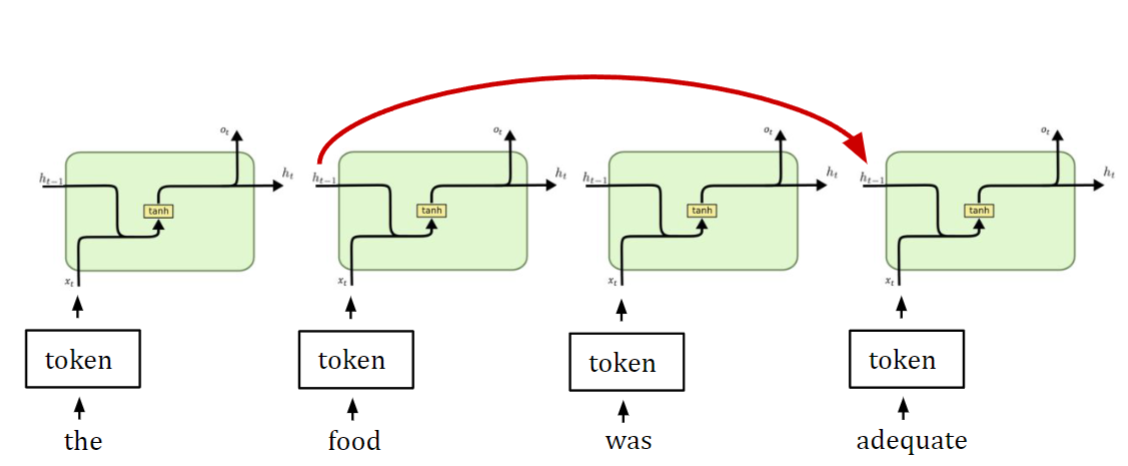
\includegraphics[width=0.75\linewidth]{skipconnection.png}
    \caption{Skip-connections for RNN}
    \label{fig:enter-label}
\end{figure}

\begin{idea}
    Vanilla RNNs lack long-term memory.
\end{idea}

\section{LSTMs \& GRUs}

\textbf{Gating Mechanism}

\begin{definition}
     \textbf{Gating Mechanism:} refers to a set of learnable components that regulate the flow of information through the network's hidden states. Gating mechanisms, such as those used in Long Short-Term Memory (LSTM) and Gated Recurrent Unit (GRU) cells, allow the network to selectively update, forget, or pass along information from previous time steps, enabling better modeling of long-term dependencies and mitigating issues like vanishing gradients.
\end{definition}

\begin{itemize}
    \item We can approximate skip-connections to all previous states by learning to \textbf{weight
previous states differently} instead (soft skip-connections)
\item We can use \textbf{gates }that learn to update the context \textbf{selectively}
\item Gating mechanism controls how much informations flows through.
\item Suppose X is a vector, then we can control how much of X to pass to next step by:
\begin{enumerate}
    \item Sigmoid or Tanh: \(f(x) = X \cdot \sigma(X)\)
    \item A neural network: \( f(x) = X \cdot NN(X) \)
\end{enumerate}
\end{itemize}

\noindent\textbf{Long Short-Term Memory (LSTM)}

\begin{figure}[h!t]
    \centering
    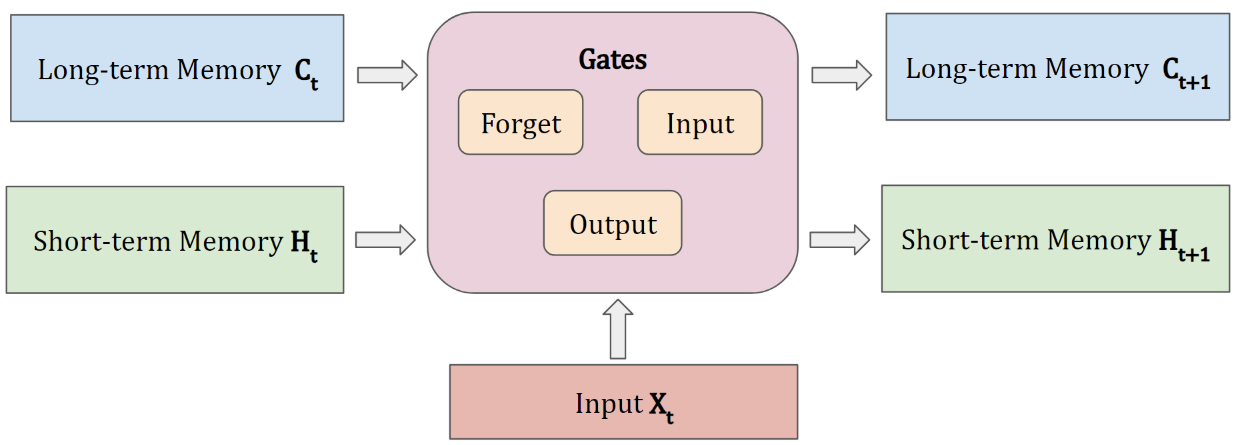
\includegraphics[width=0.65\linewidth]{lstm.png}
    \caption{LSTM}
    \label{fig:enter-label}
\end{figure}

\begin{definition}
    \textbf{Long Short-Term Memory:} a type of recurrent neural network (RNN) architecture designed to model sequential data by effectively capturing and preserving long-term dependencies. LSTMs use a specialized cell with gating mechanisms to control the flow of information, allowing them to store, update, and retrieve information over extended sequences, making them well-suited for tasks involving sequences, such as natural language processing and time series analysis.
\end{definition}


\begin{itemize}
    \item LSTMs consist of a \textbf{long-term memory} (cell state) and a \textbf{short-term memory} (context
or hidden state)
\item They use three gates to update the memories:
\end{itemize}

\begin{enumerate}
    \item \textbf{Forget Gate} (long-term memory) → How much of the past memory should we forget?

\begin{figure}[h!t]
    \centering
    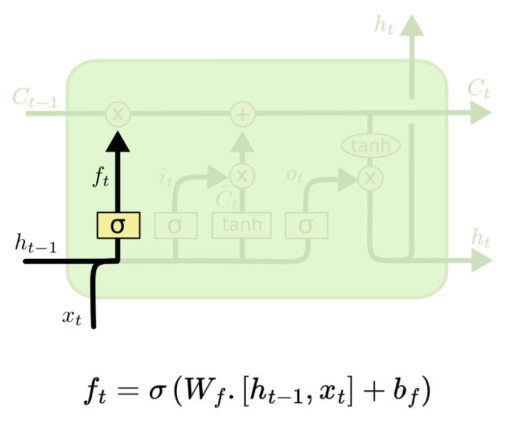
\includegraphics[width=0.4\linewidth]{forgetgate.png}
    \caption{Forget Gate}
    \label{fig:enter-label}
\end{figure}

    \item \textbf{Input Gate }(long-term memory)→ How much the current input should contribute to
the memory?
\begin{enumerate}
    \item The updated long-term memory is the amount of past that is remembered (decided by forget gate) combined with the memory that was just created (decided by input gate)

\begin{figure}[h!t]
    \centering
    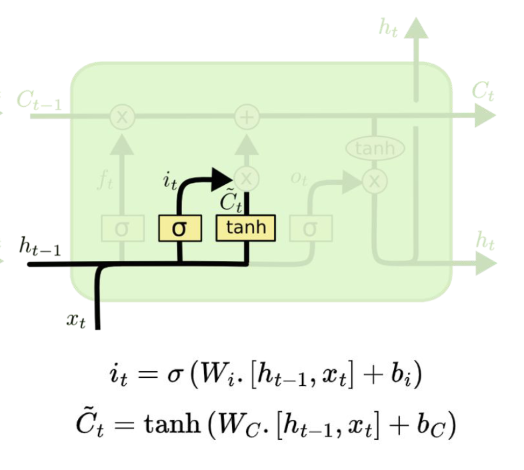
\includegraphics[width=0.4\linewidth]{inputgate.png}
    \caption{Input Gate}
    \label{fig:enter-label}
\end{figure}
\newpage
\begin{figure}[h!t]
    \centering
    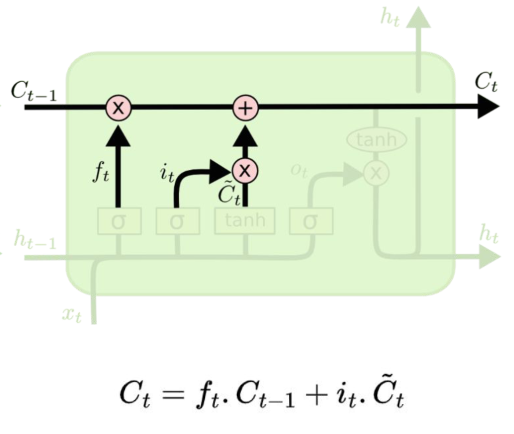
\includegraphics[width=0.4\linewidth]{updatedlongterm.png}
    \caption{Updated long-term memory}
    \label{fig:enter-label}
\end{figure}

\end{enumerate}
\item \textbf{Output Gate} (short-term memory) → How much of the updated long-term memory
should construct the short-term memory?
\end{enumerate}

\begin{figure}[h!t]
    \centering
    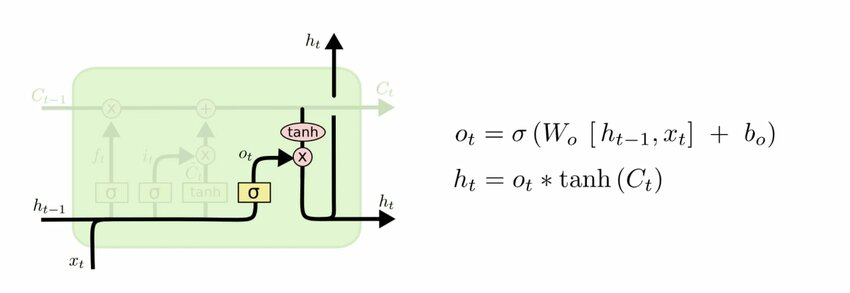
\includegraphics[width=0.8\linewidth]{outputgate.png}
    \caption{Output Gate}
    \label{fig:enter-label}
\end{figure}

\textbf{Gated Recurrent Unit (GRU)}

\begin{figure}[h!t]
    \centering
    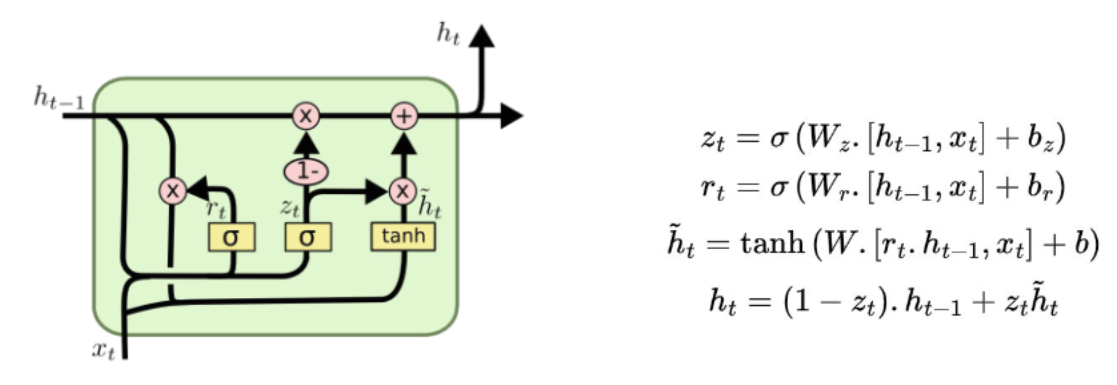
\includegraphics[width=0.75\linewidth]{GRU.png}
    \caption{GRU}
    \label{fig:enter-label}
\end{figure}

\begin{definition}
    \textbf{Gated Recurrent Unit:} a type of recurrent neural network (RNN) architecture that is designed for modeling sequential data. It simplifies the architecture of Long Short-Term Memory (LSTM) networks by using fewer gates but still effectively captures and manages information over time. GRUs have gate mechanisms that control the flow of information, helping them mitigate the vanishing gradient problem and enabling the modeling of long-term dependencies in sequential data, making them suitable for various tasks such as natural language processing and time series analysis.
\end{definition}

\begin{itemize}
    \item GRUs are more efficient than LSTMs while having similar performance
    \item They combine \textbf{forget and input gates} into an \textbf{update gate}
    \item They also merge cell state and hidden state\\
\end{itemize}

\textbf{LSTM/GRU vs RNN}

\begin{figure}[h!t]
    \centering
    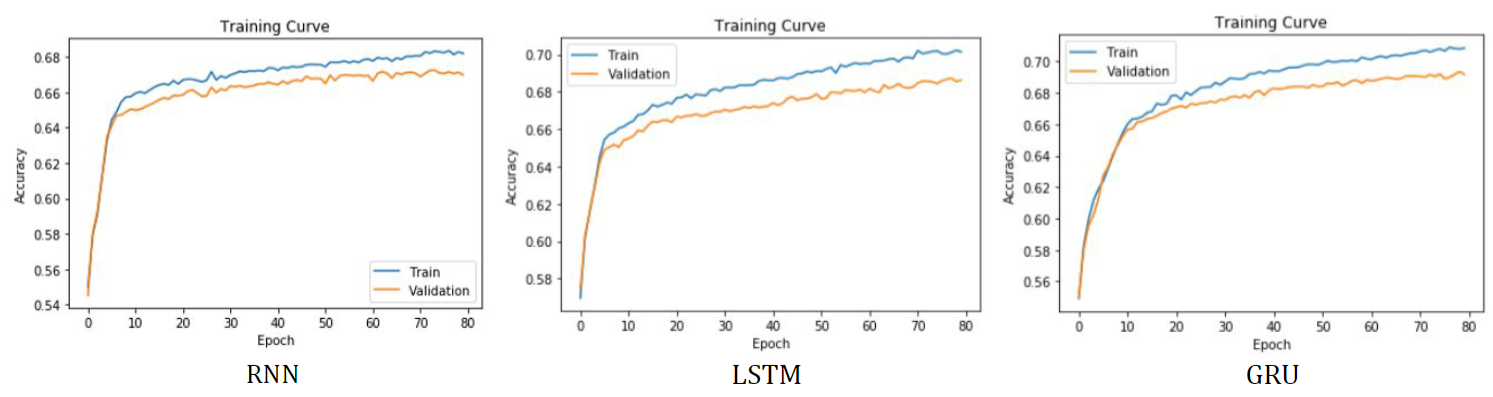
\includegraphics[width=1\linewidth]{lstmgrurnn.png}
    \caption{LSTM/GRU vs RNN}
    \label{fig:enter-label}
\end{figure}

\begin{itemize}
    \item LSTMs/GRUs can be trained on longer sequences and are much better at learning
long-term relationships
\item They are easier to train and achieve better performance than vanilla RNNs
\item LSTM/GRU haven't finished converging here, with more training they do better
\end{itemize}

\begin{figure}[h!t]
    \centering
    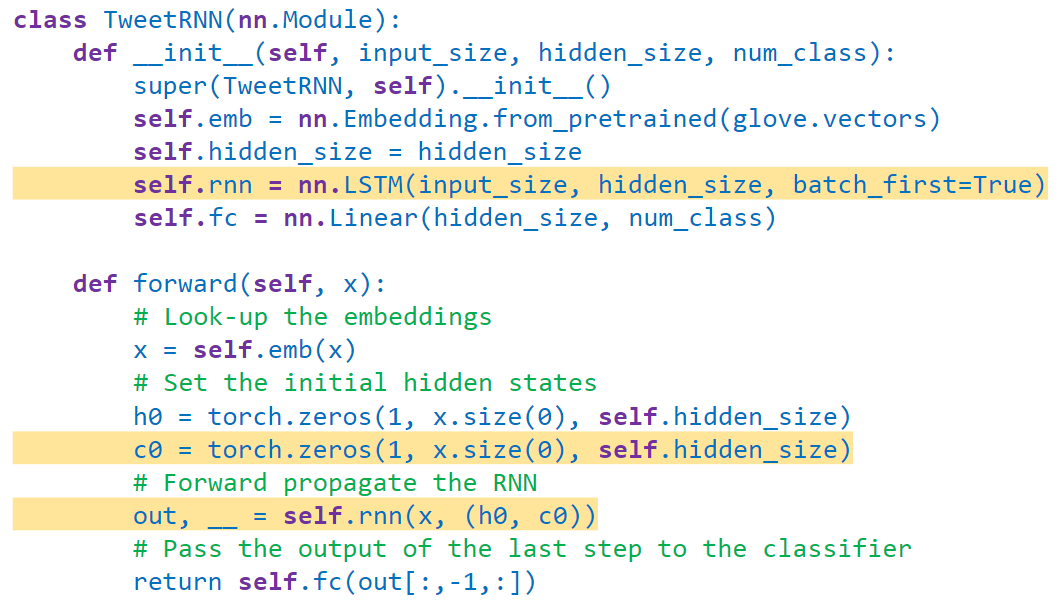
\includegraphics[width=0.65\linewidth]{lstmpy.png}
    \caption{PyTorch implementation of vanilla RNN}
    \label{fig:enter-label}
\end{figure}
\begin{figure}[h!t]
    \centering
    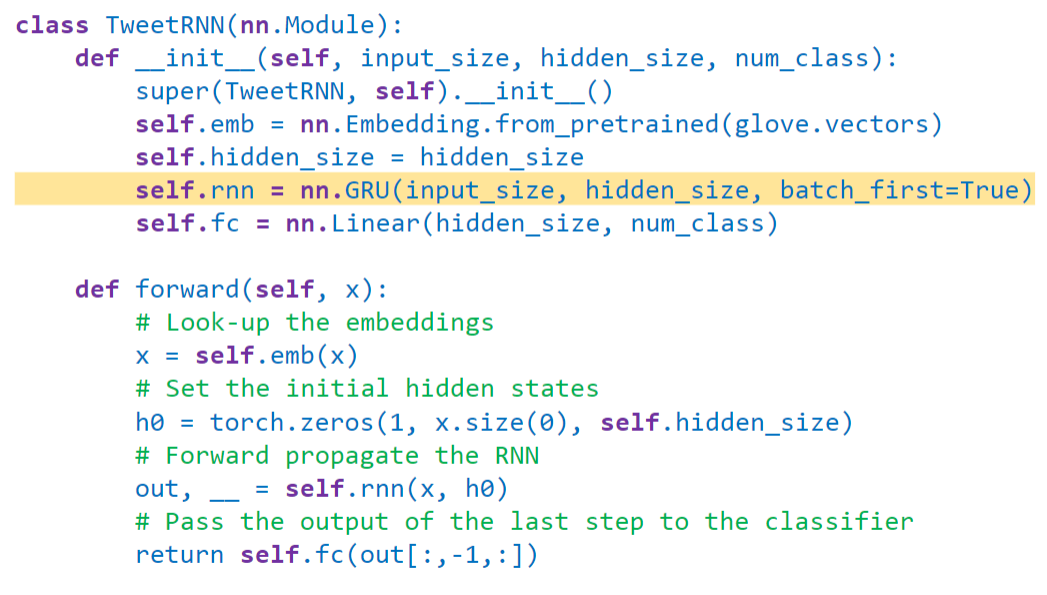
\includegraphics[width=0.65\linewidth]{grupy.png}
    \caption{PyTorch implementation of GRU RNN}
    \label{fig:enter-label}
\end{figure}
\begin{figure}[h!t]
    \centering
    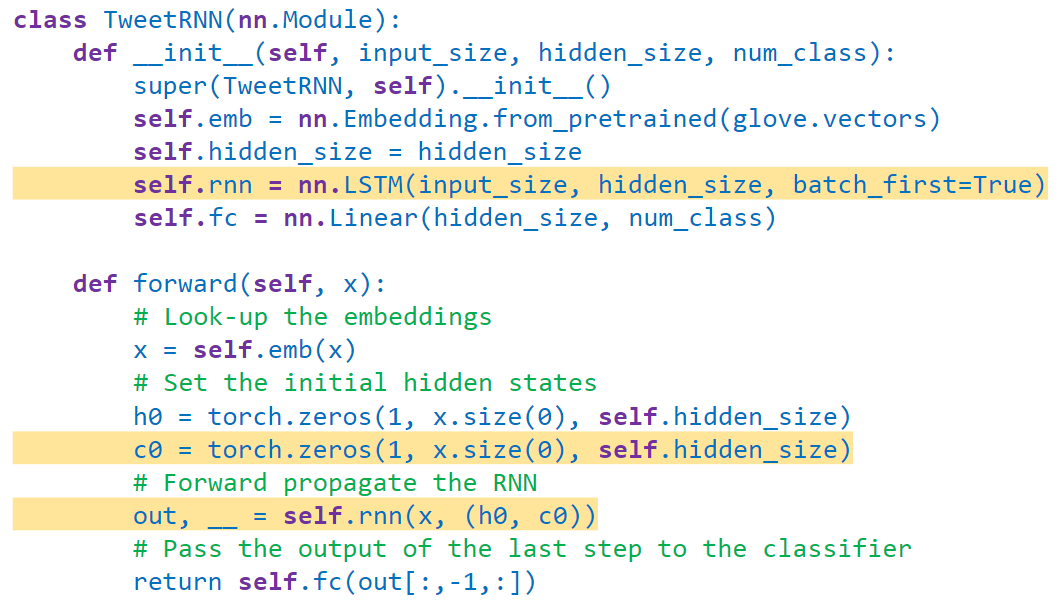
\includegraphics[width=0.65\linewidth]{lstmpy.png}
    \caption{PyTorch Implementation of LSTM RNN}
    \label{fig:enter-label}
\end{figure}

\section{Deep \& Bidirectional RNNs}

\textbf{Bidirectional RNNs}

\begin{figure}[h!t]
    \centering
    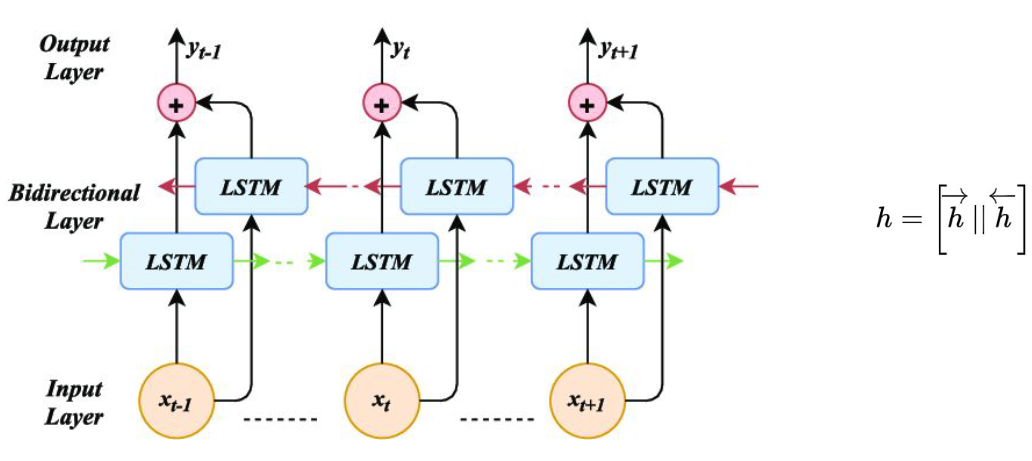
\includegraphics[width=0.8\linewidth]{bidirectional.png}
    \caption{Bidirectional RNN}
    \label{fig:enter-label}
\end{figure}

\begin{definition}
    \textbf{Bidirectional RNN:} a type of neural network architecture that processes input sequences in both forward and reverse directions simultaneously. This allows them to capture information from past and future time steps, making them particularly useful for tasks where context from both directions is essential, such as natural language understanding and speech recognition.
\end{definition}

\begin{itemize}
    \item A typical state in an RNN (RNN, GRU, or LSTM) relies on the past and the present.
    \item In tasks such as machine translation, where a prediction depends on the past,
present, and future, we can exploit the future to improve performance.

\end{itemize}

\newpage

\textbf{Deep RNNs}

\begin{figure}[h!t]
    \centering
    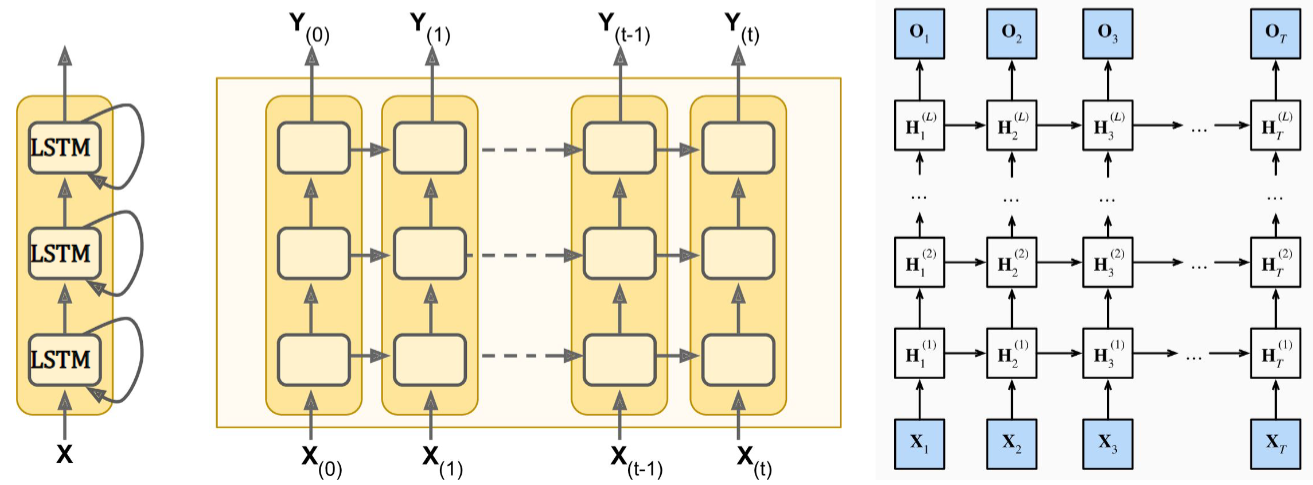
\includegraphics[width=0.8\linewidth]{deeprnn.png}
    \caption{Deep RNN}
    \label{fig:enter-label}
\end{figure}

\begin{definition}
    \textbf{Deep RNN:}  a type of recurrent neural network architecture that consists of multiple recurrent layers stacked on top of each other. These additional layers enable the network to capture more complex hierarchical features and representations from sequential data, making them suitable for tasks that require a deep understanding of temporal dependencies and context.
\end{definition}

\begin{itemize}
    \item We can also stack RNN layers to learn more abstract representations.
    \item Representations in first layers are better for syntactic tasks (low level) while representations in
last layers perform better on semantic tasks (high level).
\end{itemize}

\begin{figure}[h!t]
    \centering
    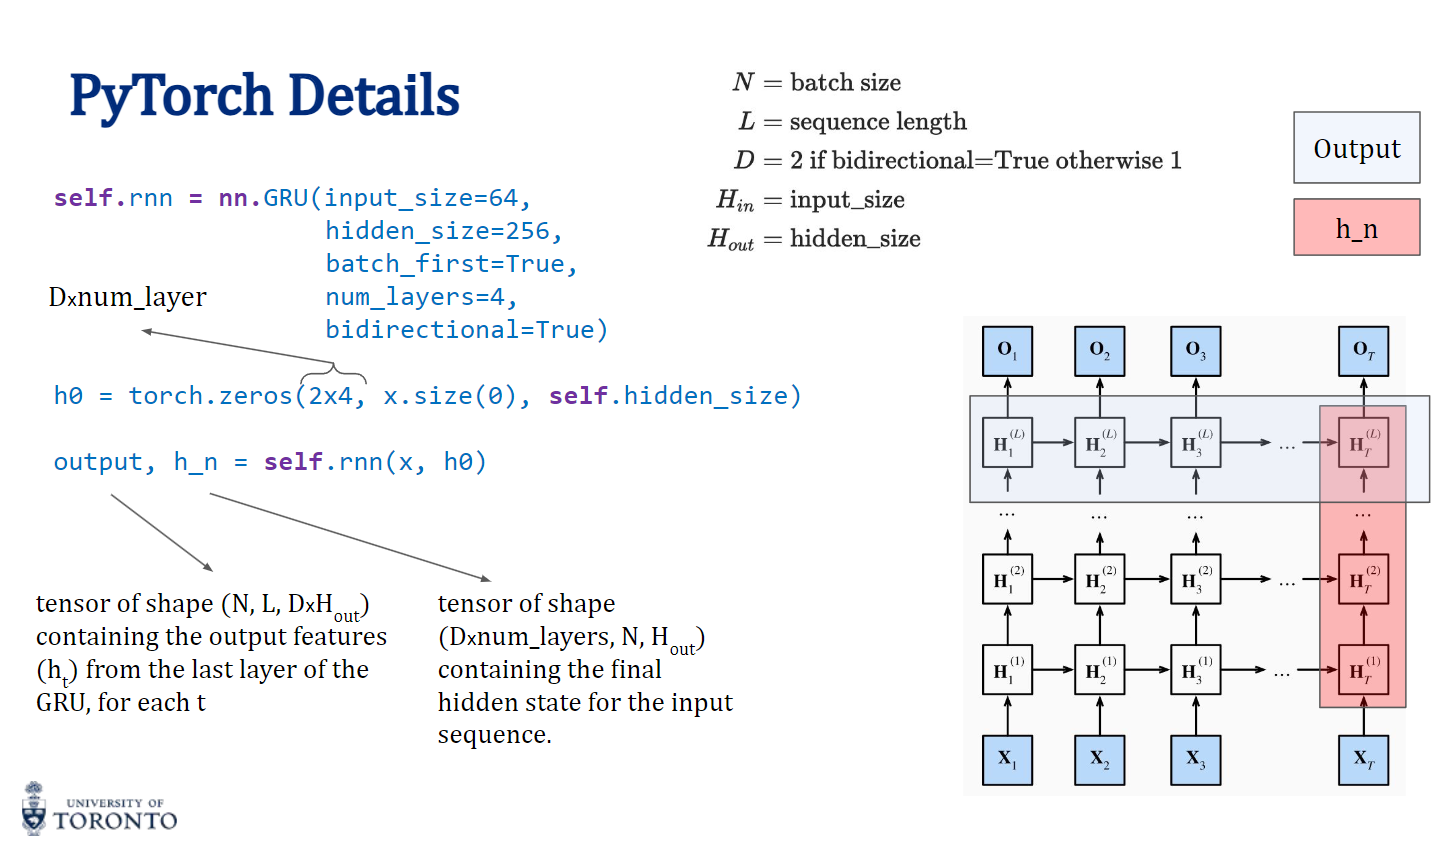
\includegraphics[width=1\linewidth]{pytorchdet.png}
    \caption{RNN configurations in PyTorch}
    \label{fig:enter-label}
\end{figure}

\newpage

\section{Sequence-to-Sequence Models}

\textbf{Sequence as input and sequence as output. }\\

\textbf{RNN Model Types}

\begin{itemize}
    \item We have focused on many-to-one and many-to-many (same length)
    \item Many other types of tasks require different slightly different RNN setups → Translation, image captioning, etc.
\end{itemize}

\begin{figure}[h!t]
    \centering
    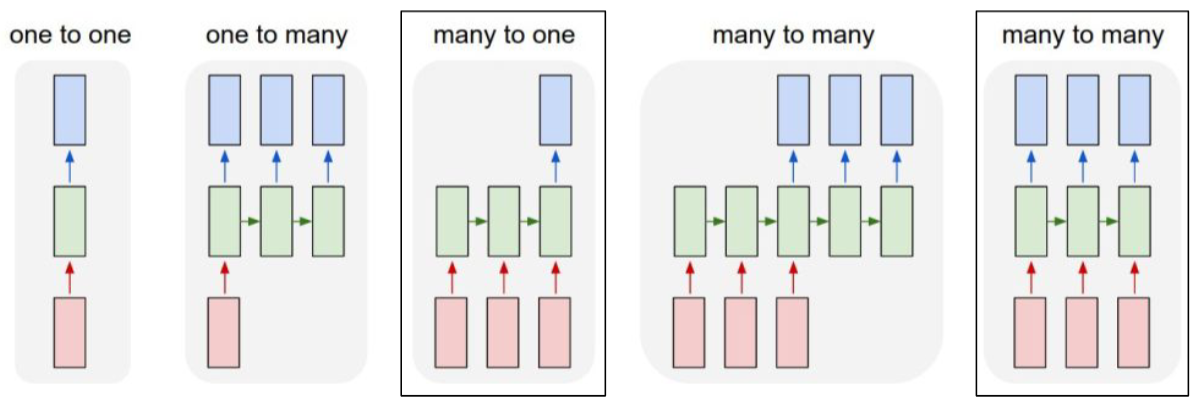
\includegraphics[width=0.75\linewidth]{rnnmodeltypes.png}
    \caption{RNN Model Types}
    \label{fig:enter-label}
\end{figure}
\newpage

\noindent\textbf{Hidden State Differences}\\

\begin{idea}
    Sequence to sequence models are actually generative. We will think of them like autoencoders.
\end{idea}

\begin{figure}[h!t]
    \centering
    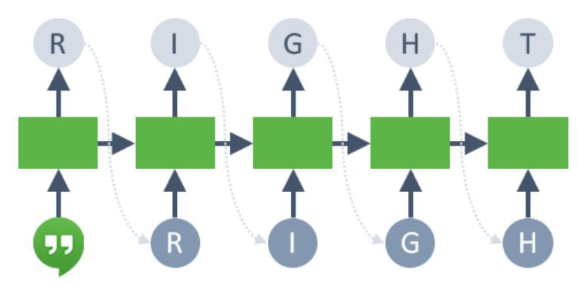
\includegraphics[width=0.65\linewidth]{right.png}
    \caption{Generating "RIGHT"}
    \label{fig:enter-label}
\end{figure}

RNNs for prediction (\textbf{Encoder})
\begin{itemize}
    \item Process tokens one at a time
    \item Hidden state represents \textbf{all the tokens read thus far}
\end{itemize}

RNNs for generating sequences (\textbf{Decoder})
\begin{itemize}
    \item Generate tokens one at a time
    \item Hidden state is a representation of \textbf{all the tokens to be generated}
\end{itemize}

\noindent \textbf{Sequence-to-Sequence RNNs}\\

Learning to generate new sequences requires addressing some problems:
\begin{enumerate}
    \item How do we generate variable-length sequences $\rightarrow$ how do we know when to \textbf{stop/finish a generated sequence!}
    \item Training-time behavior must be changed (\textbf{teacher-forcing})
    \begin{itemize}
        \item Recall added "randomness" in variational autoencoders
    \end{itemize}
    \item Inference-time behavior also changes (\textbf{sampling and temperature scaling})
\end{enumerate}

\noindent \textbf{During Training}\\

How do we know when to stop/finish a generated sequence? Let’s use dedicated control symbols to define the Beginning of Sequence \textless \textbf{BOS}\textgreater\ and End of Sequence \textless \textbf{EOS}\textgreater.\\

\textless BOS\textgreater\ R I G H T \textless EOS\textgreater\\

Once the RNN generates \textless EOS\textgreater, we will know it is done generating!\\

How to define the \textbf{ground-truth and loss}? RNN is trained to generate one particular sequence in the training set:
\begin{itemize}
    \item We feed the RNN with \textless BOS\textgreater\ and compare its prediction with R (\textbf{Cross-Entropy})
    \item We then feed it with R and compare the prediction with I
    \item $\ldots$
    \item Finally, we feed it with T and compare the prediction with \textless EOS\textgreater\\
\end{itemize}

\noindent \textbf{Teacher Forcing}\\

In each step, we compute the loss by comparing ground-truth and predicted tokens.
In order to make training more \textbf{efficient}, we force the RNN to stay close to the
ground-truth sequence.
We do this by passing the \textbf{ground-truth label as the next input} instead of current
prediction. This trick is known as \textbf{Teacher Forcing}.\\

\noindent \textbf{During Inference} \\

Unlike in a classification problem, always selecting the token with the \textbf{highest probability} won't work well:
\begin{itemize}
    \item When using a generative model, we want \textbf{diversity}, not deterministic behavior.
    \item In practice, this greedy approach results in lots of \textbf{grammatical errors}.
\end{itemize}

To address this, we \textbf{sample from the predicted distributions}. We will address 3 sampling strategies:
\begin{itemize}
    \item \textbf{Greedy search}

\begin{definition}
    \textbf{Greedy Search:}  selects the token with highest probability as the generated token.

\[ maxp(t_1, t_2,...t_n) = maxp(t_1) \cdot p(t_2) \cdot ... \cdot p(t_n) \]

\end{definition}

    \item \textbf{Beam search}

\begin{figure}[h!t]
    \centering
    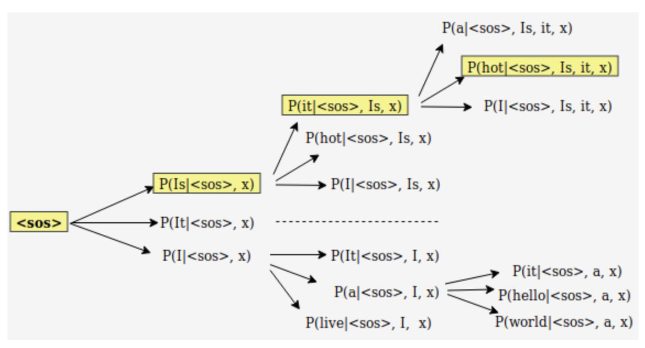
\includegraphics[width=0.75\linewidth]{beamsearch.png}
    \caption{Beam Search}
    \label{fig:enter-label}
\end{figure}

\begin{definition}
    \textbf{Beam Search:} looks for a sequence of tokens with the highest probability within a
window.

\[ maxp(t_1, t_2,...t_n) = maxp(t_1) \cdot p(t_2 | t_1) \cdot ... \cdot p(t_n|t_{n-1}, ..., t_2,t_1) \]

\end{definition}

    \item \textbf{Softmax Temperature Scaling}

\begin{figure}[h!t]
    \centering
    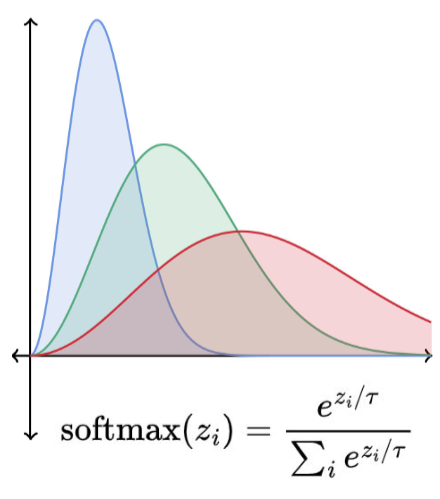
\includegraphics[width=0.4\linewidth]{softmaxtempscaling.png}
    \caption{Softmax Temperature Scaling}
    \label{fig:enter-label}
\end{figure}

\begin{definition}
    \textbf{Softmax Temperature Scaling:}  helps with the problem of over-confidence in neural
networks by by scaling the input logits to the softmax with a temperature.
\end{definition}

    \begin{itemize}
        \item \textbf{Low Temperature} (larger logits, more confident): Higher quality samples, less variety
        \item \textbf{High Temperature} (smaller logits, less confident): Lower quality samples, more variety
    \end{itemize}
\end{itemize}

\begin{figure}[h!t]
    \centering
    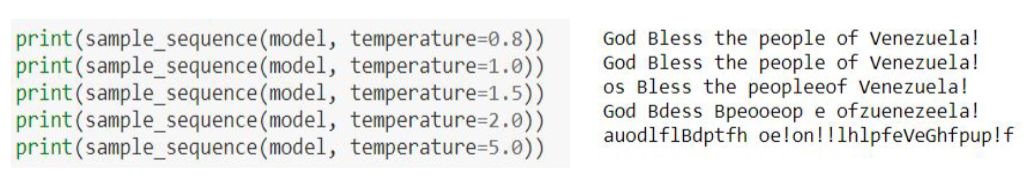
\includegraphics[width=1\linewidth]{tempscaling.png}
    \caption{Various temperature scaling configurations}
    \label{fig:enter-label}
\end{figure}

\begin{figure}[h!t]
    \centering
    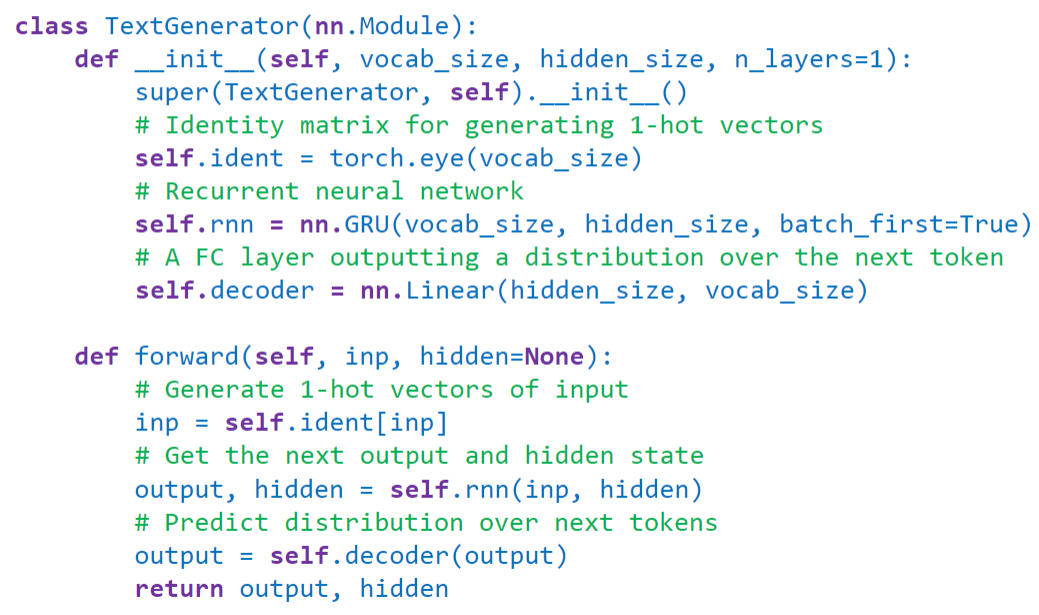
\includegraphics[width=0.655\linewidth]{textgen.png}
    \caption{Text Generator in PyTorch}
    \label{fig:enter-label}
\end{figure}
\begin{figure}[h!t]
    \centering
    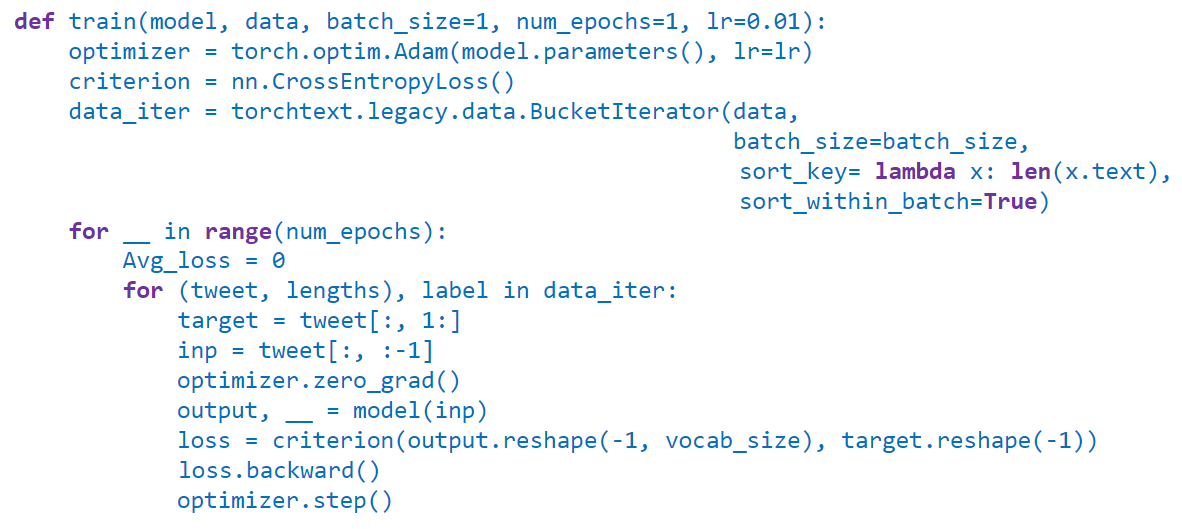
\includegraphics[width=0.8\linewidth]{traintextgen.png}
    \caption{Training the text generator}
    \label{fig:enter-label}
\end{figure}
\begin{figure}[h!t]
    \centering
    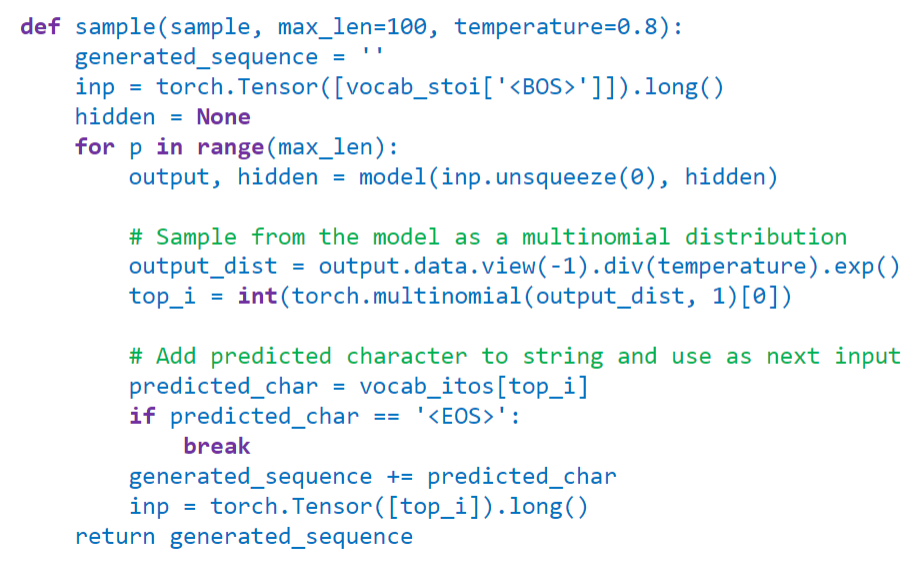
\includegraphics[width=0.655\linewidth]{samplingtextgen.png}
    \caption{Sampling the text generator}
    \label{fig:enter-label}
\end{figure}

\begin{idea}
    Language models and sequence-to-sequence models are self-supervised.
\end{idea}

\newpage

